\section{Finite-element discretization}

\subsection{Heat pump discretization}

Het algemene model van de warmtepomp en airco wordt afgeleid met behulp van het volgende geschematiseerde black box model:

\subsection{Buffer vessel discretization}

Als voorbeeld van een model met warmtestromen en warmtediffusie wordt het volgende model van
een buffervat beschouwd:

\begin{figure}[H]
	\centering
	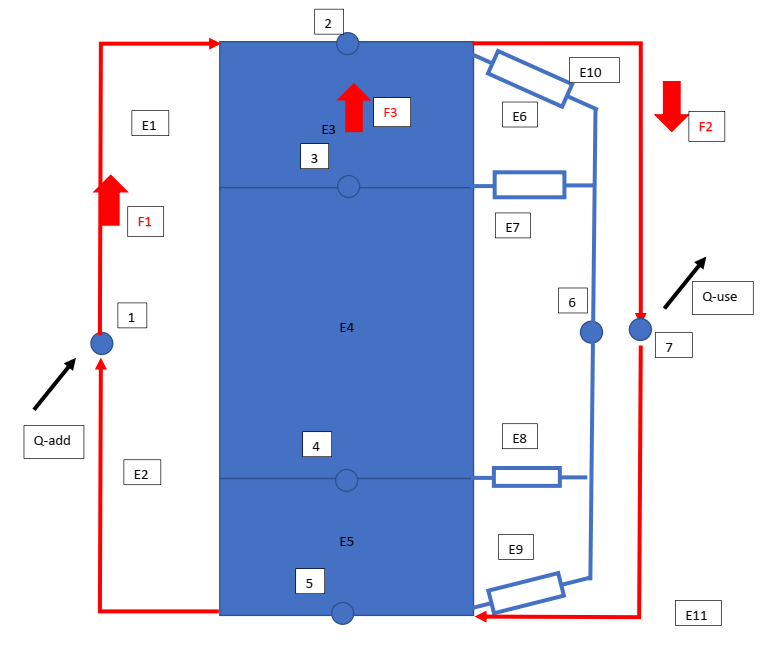
\includegraphics[width=0.7\columnwidth]{Pictures/FEwatervat.png}
	\caption[Short title]{Finite-element buffer vessel}
	\label{fig:FEbuffervessel}
\end{figure}

Dit is een buffervat in een verwarmingsinstallatie.

Voor het modelleren hiervan wordt gebruik gemaakt van een tweetal universele elementen:

\begin{enumerate}
	\item Exchange element. Dit element beschrijft warmtetransportt via een vloeistofstroom $F$ door het element en warmtetransport door geleiding. Het element kan een warmtecapaciteit
	hebben.
	\item Een puntbron. Deze bron beschrijft warmteontwikkeling of warmte-onttrekking in een punt.
\end{enumerate}

Het vat is verdeeld in 3 niveaus over de hoogte:
\begin{enumerate}
	\item Bovenzijde vat (element 3)
	\item Midden vat( element 4 )
	\item Onderzijde vat (element 5 )
\end{enumerate}

In het vat is sprake van:
\begin{itemize}
	\item Warmteverlies naar andere temperatuurniveau ’s en naar de omgeving. De
	omgevingstemperatuur in dit model is gegeven door de temperatuur in punt 7.
	De elementen die het volume van het vat beschrijven (E3,E4 en E5) wisselen warmte uit naar
	elkaar en naar punt 6.
	\item Warmtetransport door waterstromen. In waterstromen buiten het vat wordt warmte
	onttrokken of toegevoegd. In het vat is een waterstroom die zorgt voor het kortsluiten van
	de kringlopen.
\end{itemize}

Deze beide mechanismen worden meegenomen in het model.

Er wordt verondersteld dat gebruik wordt gemaakt van gelaagdheid. Boven in het vat heerst een
hogere temperatuur dan onderin het vat. Daarnaast is er sprake van een tweetal leidingen waarin
warmte wordt uitgewisseld met de omgeving:

\begin{itemize}
	\item Een leiding waarin warmte wordt toegevoegd aan het vat $\dot{Q}_{add}$. Deze leiding neemt
	vloeistof (water) onder uit het vat (punt 5), verhoogt de temperatuur door warmte-inbreng
	(punt 1) en brengt het water boven in het vat weer in. Deze leiding bestaat uit de
	elementen E1 (boven) en E2 (onder). In deze leiding is een vloeistofstroom $F_1 (kJ/(K·s))$
	aanwezig die de warmte transporteert.
	\item Een leiding waarin warmte wordt onttrokken aan het vat $\dot{Q}_{use}$. Deze leiding neemt vloeistof (water) boven uit het vat (punt 2), verlaagt de temperatuur door warmteonttrekking (punt 7) en brengt het water boven in het vat weer in. Deze leiding bestaat uit	de elementen E10 (boven) en E11 (onder). In deze leiding is een vloeistofstroom $F_2 (kJ/(K·s))$ aanwezig die de warmte transporteert.
\end{itemize}

\subsection{Matrixvergelijking}

Voor het oplossen van de temperatuurverdeling wordt per knooppunt een energiebalans opgesteld.
Deze energiebalans resulteert in een matrixvergelijking.

\begin{equation}
	\begin{aligned}
	    \mathbf{K \theta + C \dot{\theta}} = \mathbf{\dot{q}}	    	
	\end{aligned}
\end{equation}

$K$: de warmtegeleidingsmatrix (W/K)
$C$: de warmtecapaciteitsmatrix (J/K)
$\theta$: de temperatuursvector (K)
$\dot{\theta}$: de tijdsafgeleide van de temperatuursvector (K/s)
$\dot{q}$: de vector met thermische brontermen (W)

\subsection{Elementen in de stroming}

Om te komen tot het matrixmodel wordt begonnen met één exchange element zoals hierboven
geïntroduceerd (E1,E2,E3,E4,E5,E10,E11). Dit element bevat 2 knooppunten. De volgende veronderstellingen worden gedaan:

\begin{itemize}
	\item Het element bevat 2 knooppunten waarmee deze verbonden is met de omgeving. De
	nummering bedraagt: $n_1$ en $n_2$.
	\item Binnen het element heerst een lineair verlopende temperatuur, van knooppunt naar
	knooppunt.
	\item Binnen het element is een vloeistofstroom $F$ die zorgt voor additioneel warmtetransport. De stroomrichting is van knooppunt 1 naar knooppunt 2.
	\item De warmtecapaciteit van het element wordt evenredig verdeeld over de knooppunten.
\end{itemize}

De warmtestroom vanuit het element naar knoopunten 1 en 2 moet in balans zijn met de andere
warmtestromen en de warmtegeneratie in de betreffende knooppunten.

\begin{figure}[H]
	\centering
	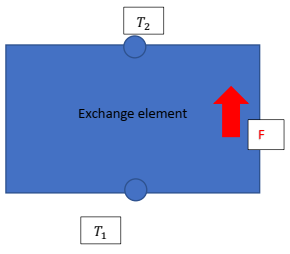
\includegraphics[width=0.7\columnwidth]{Pictures/exchange_element.png}
	\caption[Short title]{Exchange element buffer vessel}
	\label{fig:exchange_element}
\end{figure}

Voor de warmtestromen vanaf knooppunt 1 geldt:

\begin{equation}
	\begin{aligned}
		(T_1 - T_2) \cdot \frac{1}{R_e} + C_{e1,1} \cdot \frac{dT_1}{dT} = \dot{Q}_{ext,1}	    	
	\end{aligned}
\end{equation}

$T_1$: temperatuur in knooppunt 1 \\
$T_2$: temperatuur in knooppunt 2 \\
$R_e$: warmteweerstand voor geleiding tussen knooppunt 1 en 2 \\
$C_{e1,1}$: warmtecapaciteit in knooppunt 1 van element 1 \\
$\frac{dT_1}{dT}$: temperatuursverandering in de tijd in knooppunt 1 \\
$\dot{Q}_{ext,1}$: externe warmtetoevoer in knooppunt 1 \\

De vloeistofstroom $F$ vanuit knooppunt $T_1$ heeft dezelfde temperatuur als $T_1$ en heeft dus geen invloed op de temperatuur in $T_1$.

Voor de warmtestromen vanaf punt 2 geldt:

\begin{equation}
	\begin{aligned}
		(T_2 - T_1) \cdot \frac{1}{R_e} + F \cdot (T_2 - T_1) + C_{e1,2} \cdot \frac{dT_2}{dT} = \dot{Q}_{ext,2}	    	
	\end{aligned}
\end{equation}

$C_{e1,2}$: warmtecapaciteit in knooppunt 2 van element 1 \\
$\frac{dT_2}{dT}$: temperatuursverandering in de tijd in knooppunt 2 \\
$\dot{Q}_{ext,2}$: externe warmtetoevoer in knooppunt 2 \\

In matrixnotatie:

\begin{equation}
	\begin{aligned}
	\begin{bmatrix}
	    1/R_e & -1/R_e \\
	    -1/R_e -F &  1/R_e + F
    \end{bmatrix}
    \cdot
    \begin{bmatrix}
    	T_1 \\
    	T_2
    \end{bmatrix}
    +
    	\begin{bmatrix}
    	C_{e1,1} & 0 \\
    	0 &  C_{e1,2}
    \end{bmatrix}
    \cdot
    \begin{bmatrix}
    	\frac{dT_1}{dt} \\
	    \frac{dT_2}{dt}
    \end{bmatrix}	
    =
        \begin{bmatrix}
    	\dot{Q}_{ext,1} \\
    	\dot{Q}_{ext,2}
    \end{bmatrix}  	
	\end{aligned}
\end{equation}

Merk op dat door de aanwezigheid van een vloeistofstroom $F$, de geleidingsmatrix niet langer symmetrisch is.

Daarnaast wordt gebruik gemaakt van elementen die alleen een warmteweerstand weergeven. Deze
elementen (E6,E7,E8 en E9) kunnen worden gerepresenteerd met de volgende matrixvergelijking

\begin{equation}
	\begin{aligned}
		\begin{bmatrix}
			1/R_e & -1/R_e \\
			-1/R_e &  1/R_e
		\end{bmatrix}
		\cdot
		\begin{bmatrix}
			T_1 \\
			T_2
		\end{bmatrix}	
		=
		\begin{bmatrix}
			\dot{Q}_{ext,1} \\
			\dot{Q}_{ext,2}
		\end{bmatrix}  	
	\end{aligned}
\end{equation}

\subsection{Systemmmatrices van het buffervat}

Er wordt nu een systeemmatrix opgesteld voor het schematisch weergegeven model. Deze
systeemmatrix wordt opgebouwd uit de verschillende elementmatrices. De noodzakelijke rang van
deze systeemmatrix is het aantal knooppunten in het warmtestroomschema minus het aantal
voorgeschreven knooppunten in dit schema. Er zijn 7 knooppunten in het model. In dit geval wordt
in punt 6 de temperatuur voorgeschreven.
Er resteren dan 6 onafhankelijke vrijheidsgraden.

\subsubsection{Capaciteitsmatrix $\mathbf{C}$}

\subsubsection{$\mathbf{\dot{q}}$-vector}

De q vector wordt gegeven door:

%\begin{equation}
\[
\begin{bmatrix}
	1 & 1 & \dot{q}_1\\
	2 & 2 & \dot{q}_2\\
	3 & 3 & \dot{q}_3\\
	4 & 4 & \dot{q}_4\\
	5 & 5 & \dot{q}_5\\
	6 & 6 & \dot{q}_6
\end{bmatrix}
\]

In knooppunten 1 en 7 is een externe heat source / heatsink aanwezig.

\[
\begin{bmatrix}
	1 & 1 & \dot{Q}_{add}\\
	2 & 2 & \dot{q}_2\\
	3 & 3 & \dot{q}_3\\
	4 & 4 & \dot{q}_4\\
	5 & 5 & \dot{q}_5\\
	6 & 7 & -\dot{Q}_{use}
\end{bmatrix}
\]

Het voorgeschreven knooppunt (randvoorwaarde, boundary condition) 6 is verbonden aan knooppunten 2, 3,4 en 5. Dit zijn de ook de vrijheidsgraden 2,3,4, en 5. Vrijheidsgraden worden aangegeven met DOF (degree of freedom). In de overeenkomstige knooppunten wordt de capaciteitsmatrix K en de bronvector q aangepast.De aanpassing van de K-matrix wordt verderop toegelicht. De bronvector  wordt als volgt aangepast:


\[
\begin{bmatrix}
	1 & 1 & \dot{Q}_{add}\\
	2 & 2 & 0 - \frac{1}{R_{2,6}}\\
	3 & 3 & 0 - \frac{1}{R_{3,6}}\\
	4 & 4 & 0 - \frac{1}{R_{4,6}}\\
	5 & 5 & 0 - \frac{1}{R_{5,6}}\\
	6 & 7 & -\dot{Q}_{use}
\end{bmatrix}
\]

\[
\begin{bmatrix}[*2cr@{\quad}|@{\quad}>{\bf\color{red}}r]
	a & b & 1  &  4 \\
	c & d & -2 & -3
\end{bmatrix}
\]
%\end{equation}

\subsubsection{Geleidingsmatrix $\mathbf{K}$}

elements with heat capacity must have two nodes:
E3, E4, E5
elements without heat capacity have two nodes as well:
E1, E2, E6, E7, E8, E9, E10, E11

nodes:
E1 has 1 and 2
E2 has 1 and 5
E3 has 2 and 3
E4 has 3 and 4
E5 has 4 and 5
E6 has 2 and 6
E7 has 3 and 6
E8 has 4 and 6
E9 has 5 and 6
E10 has 2 and 7
E11 has 5 and 7

edges conductivity R and convection F:

1 and 2
1 and 5
2 and 3
3 and 4
4 and 5
2 and 6
3 and 6
4 and 6
5 and 6
2 and 7
5 and 7

\[
\begin{bmatrix}
	1 & 1 & \dot{Q}_{add}\\
	2 & 2 & 0 - \frac{1}{R_{2,6}}\\
	3 & 3 & 0 - \frac{1}{R_{3,6}}\\
	4 & 4 & 0 - \frac{1}{R_{4,6}}\\
	5 & 5 & 0 - \frac{1}{R_{5,6}}\\
	6 & 7 & -\dot{Q}_{use}
\end{bmatrix}
\]

\newpage